% modified from http://texample.net/tikz/examples/state-machine/

\documentclass{article}

\usepackage{tikz}
\usetikzlibrary{arrows,automata}

\begin{document}

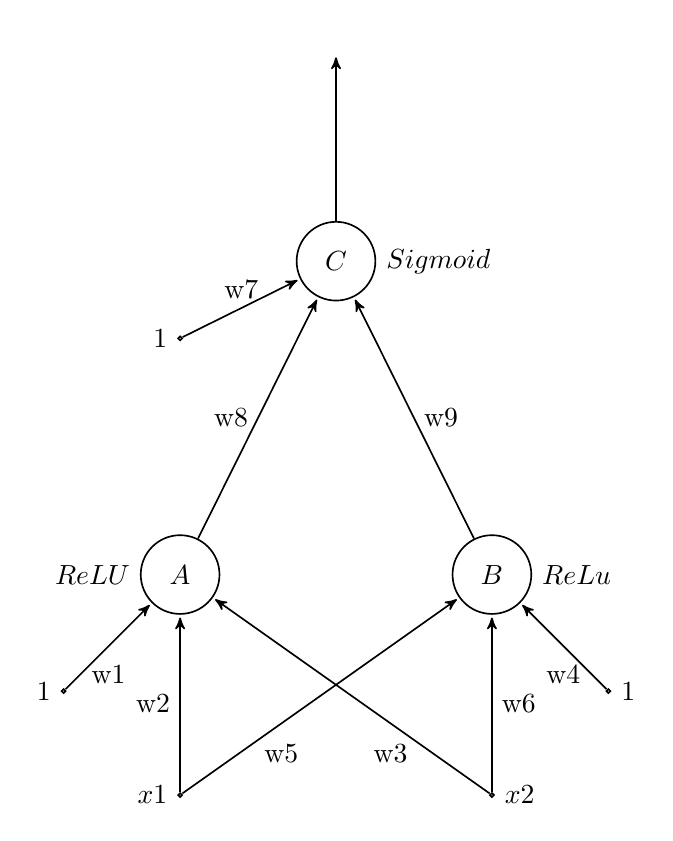
\begin{tikzpicture}[->,>=stealth',shorten >=1pt,auto,node distance=2.8cm,
                    semithick]
  \tikzstyle{state}=[circle,draw=black,text=black,minimum size=1cm]
  \tikzstyle{point}=[circle,draw=black,text=black,inner sep=0pt, minimum size=0.5mm]

  \node[state]         (A) [label=left:$ReLU$] {$A$};
  \node[state]         (C) [above right of=A, yshift=2cm, label=right:$Sigmoid$] {$C$};
  \node[state]         (B) [below right of=C, yshift=-2cm, label=right:$ReLu$] {$B$};
  \node[point]         (X1) [below of=A,label=left:$x1$] {};
  \node[point]         (X2) [below of=B,label=right:$x2$] {};
  \node[point]         (Y1) [below left of=A, xshift=0.5cm, yshift=0.5cm, label=left:$1$] {};
  \node[point]         (Y2) [below right of=B, xshift=-0.5cm, yshift=0.5cm, label=right:$1$] {};
  \node[point]         (Y3) [below left of=C, yshift=1cm, label=left:$1$] {};
  \node[circle]        (Z) [above of=C] {};




  \path (A) edge              node [left] {w8} (C)
        (B) edge              node [right] {w9} (C)
        (C) edge              node {} (Z)
        (X1) edge             node {w2} (A)
             edge             node [below, xshift=-0.5cm, yshift=-0.5cm] {w5} (B)
        (X2) edge             node [below, xshift=0.5cm, yshift=-0.5cm] {w3} (A)
             edge             node [right] {w6} (B)
        (Y1) edge             node [above, yshift=-6mm] {w1} (A)
        (Y2) edge             node [above, yshift=-6mm] {w4} (B)
        (Y3) edge             node [above] {w7} (C);
\end{tikzpicture}

\end{document}
